\section{Correlation Between Ratings and Product Descriptions}

\begin{frame}{Overview}
	% \frametitle<presentation>{Overview}
    
	\begin{block}{1. Visual Information Correlation}
		\begin{itemize}
			\item Correlation with the number of sample images
		\end{itemize}
	\end{block}
    
	\begin{block}{2. Text Information Correlation}
		\begin{itemize}
			\item Correlation with description length
			\item Correlation with reading ease
			\item Correlation with the marketing tone of the description
            \item Correlation with product description items
            \emph{beamerarticle}
		\end{itemize}
	\end{block}

    \textbf{Correlation computation:} We use spearmanr to compute Correlation
\end{frame}

\begin{frame}{Rating features}

	\begin{figure}
		\centering
			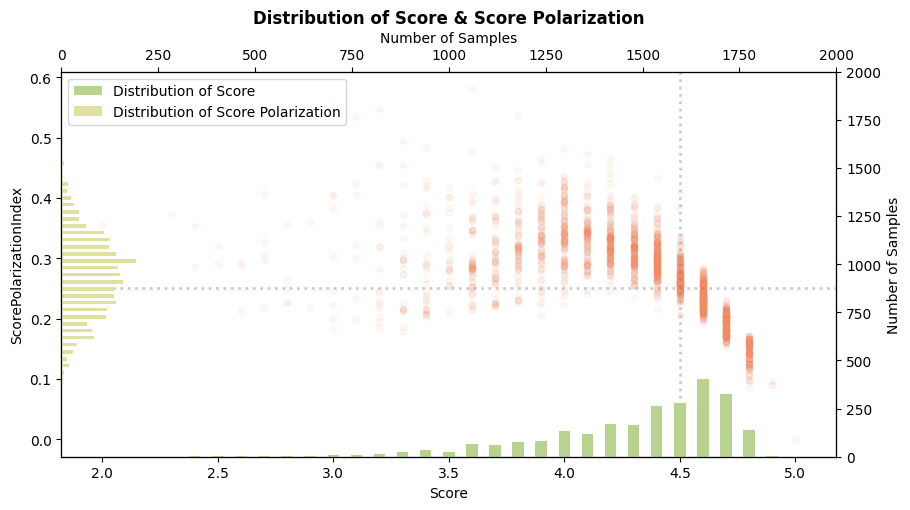
\includegraphics[height=5cm]{pic/score-scatter.png}
		% \caption{Logo of the university.}
		% \label{fig:unilogo}
	\end{figure}

    \begin{enumerate}
        \item \textbf{Mean Score:} The score displayed on the product detail page.
        \item \textbf{Score Polarization:} Indicates whether the ratings for this product are polarized.
        \item \textbf{Standards of Good Score:} Score >= 4.5; Polarization <= 0.25
    \end{enumerate}

\end{frame}
